\chapter[SCP-188 匠人]{
    SCP-188 The Craftsman\\
    SCP-188 匠人
}

\label{chap:SCP-188}

\begin{figure}[H]
    \centering
    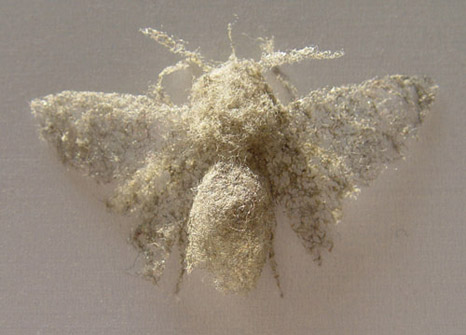
\includegraphics[width=0.5\linewidth]{images/SCP-188.jpg}
    \caption*{一个SCP-188效应的示例}
\end{figure}

\bb{项目编号:}SCP-188

\bb{项目等级:}Safe

\bb{特殊收容措施:}鉴于SCP-188没有对任何基金会资产表现出直接威胁,SCP-188应当被收容于J6-455储藏单元(Storage Unit J6-455)之中。该项目的状态应当在每两周进行一次的基金会资产调查中得到记录。在此期间,任何由SCP-188对环境产生的影响都应当被抹消。

\bb{描述:}SCP-188是一定量的金属铱,能在周围有限范围内事物上产生某种效应。如果不考虑这种范围性效应,无论是在物理性质上还是化学性质上,SCP-188与寻常的金属铱都别无二致。SCP-188的质量为一百八十一点四三克(181.43 g),被铸成了圆柱状,其半径为一厘米(1 cm),长度为二点五六厘米(2.56 cm)。SCP-188目前的圆柱体形态并非其原始状态,仅是基金会人员考虑到实验处理和收容操作的便利而作的改变。

SCP-188所产生的范围性效应可改变外界环境。这些改变体现为一些非连续的操作,如刮擦物体表面,以及对以尘土为代表的周围物质的聚集和塑形。这些变化会随时间积累,并在影响区域内扩散,展现高度的复杂性和精巧的构造,且被观察到渐变的过程。进一步地,该效应在每一个尺度上产生,产生的构造也变得极其微小和复杂。最初被基金会收容的时候,SCP-188持续地构造着分形纹样。自被收容以来,项目渐渐转而制造螺旋形和水波形的花纹。生物的图样虽稀有,却贯穿始终。

周边环境被影响后,SCP-188的范围性效应会向外拓展。测试表明该范围最多只会包括四千平方米(4000 m\textsuperscript{2})的区域。

将SCP-188无效化的尝试包括将之置入法拉第笼、置入辐射防护设备、研磨成粉末及熔化。以上所有措施都没能在任何层面上削弱SCP-188产生的效应。近期将SCP-188升华并重新凝结部分气体的提议正在探索中。

SCP-188在一九二█年█月█日(██\slash ██\slash 192█)第一次引起了属于印第安纳州乡村█████ ████████产权的一个基金会前身的注意。在一次彻底的搜查之后,项目以一根部分没入地下的尖刺的形态被发现,且似乎处在将当地的作物小麦编织在一起及压平麦秆以进行塑形的进程中。到获取项目为止并没有观察到明晰的图案,然而数米范围内都有效应的产生。即便记录并不完整,仍然可以获知遏制该效应的努力失败了。将项目嵌入包括混凝土和铅的大量物体也没能缩小效应最初产生的范围。更甚,项目曾割裂包裹它的封套。基金会考证到,更多涉及秘传的方法曾被建议施用,比如将之封入金刚石。并没有证据表明这些操作困难、耗资巨大的方法曾被采用。

在该前体组织并入基金会之后,该项目及其所有记录也被继承,并得到SCP-188的编号。“麦田圈”热潮涌起的时候,基金会努力地试图寻找其成因与SCP-188所引起的效应的联系。调查表明,除了表象,二者没有任何关联,O5级人员认为该相似性只是一个巧合。

调查及阐明SCP-188对其周遭环境影响在统计学上的一致性的提议已被通过,正在接受评估。目前,由于SCP-188对其现有收容措施表现出固有的威胁,不提倡要求采用极端措施或与其它SCP互动的提议。
